\documentclass{beamer}
%\documentclass[handout,t]{beamer}

\batchmode
% \usepackage{pgfpages}
\usepackage{tikz}
% \usetikzlibrary{patterns}
% \usetikzlibrary{matrix}
% \usetikzlibrary{graphs}
% \usetikzlibrary {chains,scopes}
% \usetikzlibrary {arrows.meta,automata,positioning}
% \pgfpagesuselayout{4 on 1}[letterpaper,landscape,border shrink=5mm]

\usepackage{amsmath,amssymb,enumerate,epsfig,bbm,calc,color,ifthen,capt-of}
\usepackage{macros}

\usetheme{Berlin}
\usecolortheme{mit}

\title{Feedback Linearizable Discretizations of Mechanical Systems using Retraction Maps} 
\subtitle{BTP Stage I Presentation}
\author{Shreyas N B}
\institute[IIT Bombay]{B. Tech, Department of Aerospace Engineering\\ IDDDP, Center for Systems and Control }
\date{\today}
\logo{
\includegraphics[height=1cm]{../Figures/iitblogo.png}}

\AtBeginSection[]
{
  \begin{frame}<beamer>
    \frametitle{Outline}
    \tableofcontents[currentsection]
  \end{frame}
}
\beamerdefaultoverlayspecification{<+->}
% -----------------------------------------------------------------------------
\begin{document}
% -----------------------------------------------------------------------------

\frame{\titlepage}

\section[Outline]{}
\begin{frame}{Outline}
  \tableofcontents
\end{frame}

% -----------------------------------------------------------------------------
\section{Introduction}

\begin{frame}{Motivation}
  Consider a continous-time nonlinear system of the form:

  \[ \dot{x}(t) = f(x(t), u(t)) \]

  The corresponding discrete-time nonlinear system is given by:
  \[ x_{k+1} = F(x_k, u_k) \]
  Assuming the following:
  \begin{enumerate}
    \item There exists a coordinate transformation $z := \varphi(x)$ and an auxiliary control $v : = \psi(x,u)$ such that $\dot{z}(t) = Az(t) + Bv(t)$ where $A, B$ are constant matrices.
    \item The discretization scheme is arbitrary.
  \end{enumerate}

\end{frame}

\begin{frame}{Motivation}

  \begin{block}{Question 1}
    Can we construct a discretization scheme such that the discrete system can also be linearized using $\varphi(x)$ and $\psi(x,u)$ similarly?
  \end{block}
  
  \begin{block}{Question 2}
    Can we extend this scheme (geometrically) to second-order nonlinear mechanical systems?
  \end{block}
  
\end{frame}


\subsection{Feedback Linearization}
\begin{frame}{Definitions}
\begin{block}{Continuous Feedback Linearization}
  A continous-time nonlinear system $\dot{x}(t) = f(x(t), u(t))$ is said to be feedback linearizable if there exists a coordinate transformation $z = \varphi(x)$ and a feedback control law $v = \psi(x,u)$ such that the transformed system is linear $\dot{z}(t) = Az(t) + Bv(t)$.
\end{block}

\begin{block}{Discrete Feedback Linearization}
  A discrete-time nonlinear system $x_{k+1} = F(x_k, u_k)$ is said to be feedback linearizable if there exists a coordinate transformation $z_k = \varphi(x_k)$ and a feedback control law $v_k = \psi(x_k,u_k)$ such that the transformed system is linear $ z_{k+1} = Az_k + Bv_k $, where $x_k = x(t_k)$.
\end{block}

\end{frame}


\begin{frame}{Observations}
  \begin{block}{Problem}
    Feedback linearizability of discrete-time systems depends on the choice of the discretization scheme.
  \end{block}

  \begin{block}{Objective}
    Given a (locally) feedback linearizable continuous-time nonlinear system, construct a discretization scheme such that the discrete-time system is also (locally) feedback linearizable.
  \end{block}

  \begin{block}{Strategy}
    We utilize the concept of \textbf{retraction maps} to construct such a discretization scheme.
  \end{block}
  
\end{frame}
% 

\subsection{Retraction and Discretization Maps}

\begin{frame}{Definition}
  We define a \textbf{retraction map} on a manifold $M$ as a smooth map $\Ret: TM \to M$, such that if $\Ret_x$ be the restriction of $\Ret$ to $T_x M$, then the following properties are satisfied:

    \begin{enumerate}
        \item $\Ret_x (0_x) = x$ where $0_x$ is the zero element of $T_x M$.
        \item $\text{D}\Ret_x (0_x ) = T_{0_x} \Ret_x = \mathbb{I}_{T_x M} $, where $\mathbb{I}_{T_x M}$ is the identity mapping on $T_x M$.
    \end{enumerate}
  
\end{frame}

\begin{frame}{Retraction Map}
\begin{figure}
  \centering
  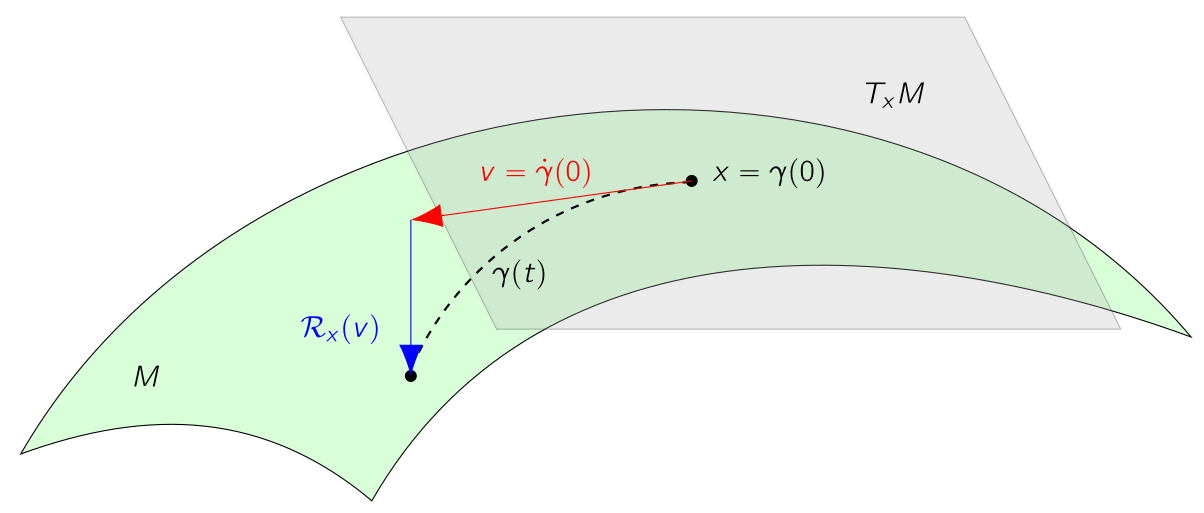
\includegraphics[width=\textwidth]{../Figures/retraction.png}
  \caption{A visualization}
\end{figure}
\end{frame}

\begin{frame}{Discretization Map}
  A map $\D : U \subset TM \longrightarrow M \times M$ given by 

\[
  \D (x,v) \equiv \D_x(v) = \left( R^1_x(v), R^2_x(v) \right)
\]

where $U$ is the open neighborhood of the zero section $0_x \in TM$, is called a \textbf{discretization map} on $M$, if the following properties are satisfied:

\begin{enumerate}
  \item $\D(x,0_x) = (x,x)$ 
  \item $T_{0_x}R_x^2 - T_{0_x}R_x^1 = \mathbb{I}_{T_x M}$, which is the identity map on $T_x M$ for any $x \in M$.
\end{enumerate}
\pause[]

\textsl{\underline{Example}: The forward Euler discretization map is given by $\D(x,v) = (x, x + v)$.}
  
\end{frame}
\section{Feedback Linearizable Discretizations}

\begin{frame}{Notations}

  \begin{itemize}
    \item $\mathfrak{X}(M)$ : set of all vector fields on $M$. 
    \item $\dot{x}(t) = X(x(t))$ : dynamical system defined by $X \in \mathfrak{X}(M)$.
    \item $\tau_M : TM \longrightarrow M$ : canonical projection $M$ s.t. $\tau_M(x,v) = x$.
    \item $h = t_{k+1} - t_k$ : time step of discretization.
    \item $\D^{TM}$ is a discretization map on $M$.
  \end{itemize}
  
\end{frame}

\subsection{Discretization of Vector Fields}
\begin{frame}{Discretization of Vector Fields}
  \begin{block}{Proposition}
    Let $X(\cdot, u_k) \in \mathfrak{X}(M)$ be a controlled vector field on $M$. Then, for a given discretization scheme $\D$,

    \[
      \D^{-1}(x_k, x_{k+1}) = hX(\tau_M(\D^{-1}(x_k, x_{k+1})), u_k)
    \]

    is an implicit numerical discretization of $\dot{x}(t) = X(x(t), u(t))$.
  \end{block}


  \begin{block}{Example}

    The forward Euler discretization scheme $\D(x,v) = (x, x + v)$ yields the explicit Euler form $x_{k+1} = x_k + hX(x_k, u_k)$.
    
  \end{block}
  
\end{frame}

\subsection{Lift of Discretization Maps}
\begin{frame}{Tangent Lift}
  \begin{block}{Proposition}
    Let $\varphi: M \lra N$ be a smooth map (diffeomorphism). For a given discretization map $\D^{TM} : TM \lra M \times M$ on $M$, the map $\D_{\varphi} :=  (\varphi \times \varphi) \circ \D^{TM} \circ T \varphi ^{-1}$ is a discretization map on $N$ i.e., $\D_{\varphi} \equiv \D^{TN} : TN \lra N \times N$.
  \end{block}

  \begin{figure}[h]
    \centering
    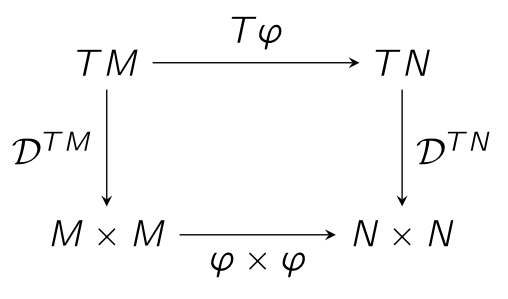
\includegraphics[width=0.5\textwidth]{../Figures/commutator.png}
  \end{figure}
\end{frame}

\begin{frame}{Feedback Linearizable Discretization}
  \begin{block}{Proposition}
    Let $\varphi$ be the linearizing coordinate transformation and $\psi$ be the linearizing feedback. Let $\D^{TN}$ be a discretization map that \textbf{discretizes the continuous-time linear system to a discrete-time linear system}. Then,

    \[
      \D^{TM} = (\varphi \times \varphi)^{-1} \circ \D^{TN} \circ T \varphi
    \]

    is a discretization on $M$ which discretizes the continuous-time system to a discrete-time nonlinear system such that the discrete-time system is feedback linearizable using $z_k : = \varphi(x_k)$ and $v_k : = \psi(x_k, u_k)$.
  \end{block}
  
\end{frame}

\section{Second-Order Mechanical Systems}

\subsection{Second-Order Differential Equations}

\begin{frame}{Discretization of SODEs}
  A second-order differential equation (SODE) is a vector field $X$ such that $\tau_{TM}(X) = T \tau_M (X)$. Locally,
  \begin{equation}
      X = \dot{x}^i \frac{\partial}{\partial x^i} + X^i(x^i, \dot{x}^i) \frac{\partial}{\partial \dot{x}^i}
  \end{equation}
  To find the integral curves of $X$ is equivalent to solving the SODE:
  \begin{equation}
  \label{eq:sode}
      \frac{d^2}{dt^2}x(t) = X \left( x(t), \frac{d}{dt}x(t) \right) 
  \end{equation}

\end{frame}

\begin{frame}{Discretization of SODEs}
  Now, we wish to discretize this using the notion of the discretization map on $TM$. We would like to tangently lift a discretization on $M$ to obtain $\D^{TTM}: TTM \lra TM \times TM$. This yields the following numerical scheme:
  \begin{equation}
  \label{eq:disc}
  \begin{split}
      h X \left( \left(\tau_{TM} \circ \left(\D^{TTM}\right)^{-1}\right)(x_k, y_k; x_{k+1}, y_{k+1})\right) \\ = \left(\D^{TTM}\right)^{-1} (x_k, y_k; x_{k+1}, y_{k+1})
  \end{split}
  \end{equation}
  
\end{frame}

\begin{frame}{What is different here?}

  The double tangent bundle $TTM$ admits two different vector bundle structures:

  \begin{enumerate}
    \item The canonical vector bundle with projection $\tau_{TM} : TTM \lra TM$.
    \item The vector bundle given by the projection of the tangent map $T \tau_M : TTM \lra TM$. 
  \end{enumerate}

  \pause
  Denote the canonical involution map $\kappa_M : TTM \lra TTM$ which is a vector bundle isomorphism, over the identity of $TM$.

\[
 \kappa_M (x, v, \dot{x}, \dot{v}) = (x,\dot{x}, v, \dot{v})
\]
  
\end{frame}

\begin{frame}{Why is this important?}
  The tangent lift of a vector field $X$ on $M$ does not define a vector field on $TM$. It is necessary to consider the composition $\kappa_M \circ TX$ to obtain a vector field on $TM$, and this is called the \textbf{complete lift} $X^c$ of the vector field $X$. 
  Hence, a similar technique must be used to lift a discretization map from $TM$ to $TTM$.

  \begin{block}{Proposition}
    If $\D^{TM} : TM \lra M \times M$ is a discretization map on $M$, then $\D^{TTM} = T\D^{TM} \circ \kappa_M$ is a discretization map on $TM$.
  \end{block}
  
\end{frame}

\begin{frame}{Tangent Lift of Discretization Map}
  \begin{figure}[h]
    \centering
    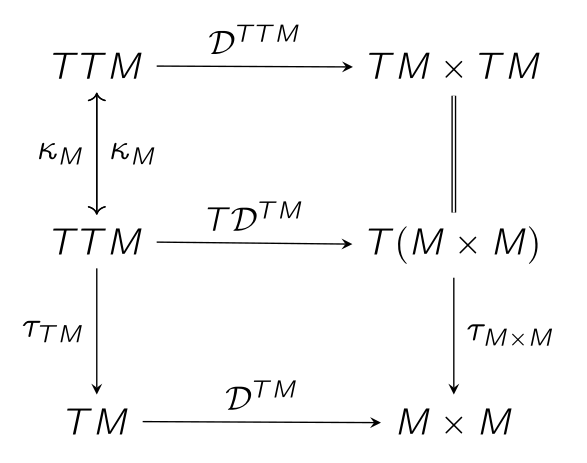
\includegraphics[width=0.5\textwidth]{../Figures/double-tangent.png}
    \caption{Commutation of maps around $TTM$}
  \end{figure}
  
\end{frame}

\begin{frame}{The whole (slightly intimidating) picture}
  \begin{figure}
    \centering
    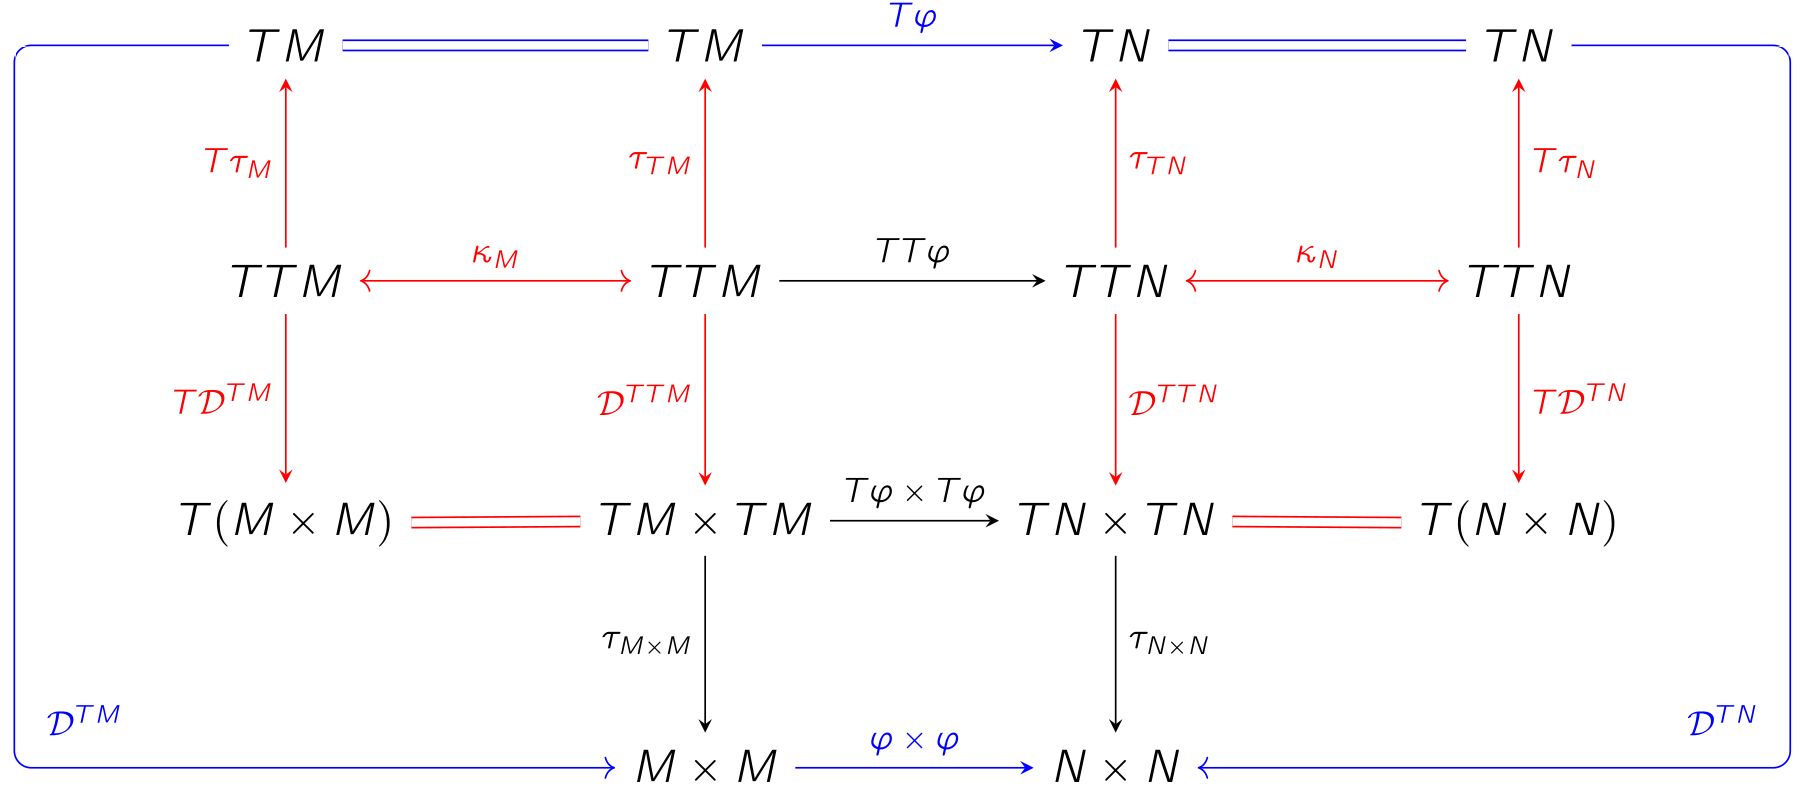
\includegraphics[width=\textwidth]{../Figures/double-commutator.png}
    \caption{The Commutator}
  \end{figure}
\end{frame}

\subsection{Mechanical Systems}

\begin{frame}{More Notation}

  \begin{itemize}
    \item $\Gamma^i_{jk}$ : Christoffel symbols (connection coefficients) on $M$.
    \item $\nabla$ : symmetric affine connection on $M$.
    \item $x = (x^1, \dots, x^i, \dots x^n)$ : local coordinates on $M$.
    \item $\mathfrak{g} = \{g_1,  \dots, g^r, \dots, g_m\}$ : control vector fields.
    \item $e$ : uncontrolled vector field.
    \item $\mathfrak{R}$ : Riemannian curvature tensor
    \item $\text{ann}$ : annihilator.
  \end{itemize}
  
\end{frame}

\begin{frame}{Definition}
  \begin{block}{Mechanical Systems}
    A mechanical control system $(\mathcal{MS})_{(n,m)}$ is defined by a $4$-tuple $(M, \nabla, \mathfrak{g}, e)$ where:
    \begin{equation}
      \label{eq:mech}
      \nabla_{\dot{x}} \dot{x} = e(x) + \sum_{r=1}^m g_r(x) u_r 
  \end{equation}
  Or equivalently in local coordinates $x = (x^1, \dots, x^n)$ on $M$, 
  \begin{equation}\label{SODE-initial}
      \ddot{x}^i = - \Gamma ^i_{jk}(x)\dot{x}^j \dot{x}^k + e^i(x) + \sum_{r=1}^m g^i_r(x)u_r
  \end{equation}
    
  \end{block}
\end{frame}

\begin{frame}{Definition}
  We can write this as two first-order differential equations:
  \begin{equation}\label{SODE-nonlinear}
      \begin{split}
          \dot{x}^i  &= y^i; \\
          \dot{y}^i  &= - \Gamma^i_{jk}(x)y^jy^k + e^i(x) + \sum_{r=1}^m g_r^i(x)u_r
      \end{split} \tag{$\mathcal{MS}$} 
  \end{equation}

  \begin{block}{Objective}
    Given a mechanical control system $(\mathcal{MS})_{(n,m)}$, we wish to construct a discretization scheme such that the discrete-time system is \textbf{mechanical feedback linearizable}.
  \end{block}
  
\end{frame}

\subsection{MF-Linearizability}

\begin{frame}{Mechanical Feedback Linearizability}
  \begin{equation*}
        \mathcal{E}^0 = \text{span} \{ g_r, 1 \leq r \leq m \} \ ; \ \mathcal{E}^j = \text{span} \{ \text{ad}^i_e g_r, 1 \leq r \leq m, 0 \leq i \leq j \}
\end{equation*}

\begin{thm}\label{thm:mfl}
    A mechanical system $(\mathcal{MS})_{(n,m)}$ is mechanical feedback ($MF$) linearizable, locally around $x_0 \in M$ iff, in the neighborhood of $x_0$:

    \begin{itemize}
        \item $(ML1)$ $\mathcal{E}^0$ and $\mathcal{E}^1$ are of constant rank
        \item $(ML2)$ $\mathcal{E}^0$ is involutive
        \item $(ML3)$ $\text{ann } \mathcal{E}^{0} \subset \text{ann } \mathfrak{R}$
        \item $(ML4)$ $\text{ann } \mathcal{E}^0 \subset \text{ann } \nabla g_r \ \forall r: 1 \leq r \leq m$
        \item $(ML5)$ $\text{ann } \mathcal{E}^1 \subset \text{ann } \nabla^2 e$
    \end{itemize}

\end{thm}
\end{frame}

\begin{frame}{Mechanical Feedback Linearizability}

For planar mechanical systems ($n=2$):

\begin{prop}
\label{prop:planar_mech}
A planar mechanical system $\mathcal{(MS)}_{(2,1)}$ is locally $MF$-linearizable at $x_0 \in M$ to a controllable $\mathcal{(LMS)}_{(2,1)}$, if and only if it satisfies the following conditions:
\begin{enumerate}
    \item $(MD1)$ $g$ and $\text{ ad}_e g$ are independent
    \item $(MD2)$ $\nabla_g g \in \mathcal{E}^0$ and $\nabla_{\text{ad}_e g} g \in \mathcal{E}^0$
    \item $(MD3)$ $\nabla^2_{g, \text{ad}_e g} \text{ad}_e g - \nabla^2_{\text{ad}_e g, g} \text{ad}_e g \in \mathcal{E}^0$
\end{enumerate}
\end{prop}
\end{frame}

\section{Results}

\begin{frame}{Inertia Pendulum}
  \begin{figure}
    \centering
    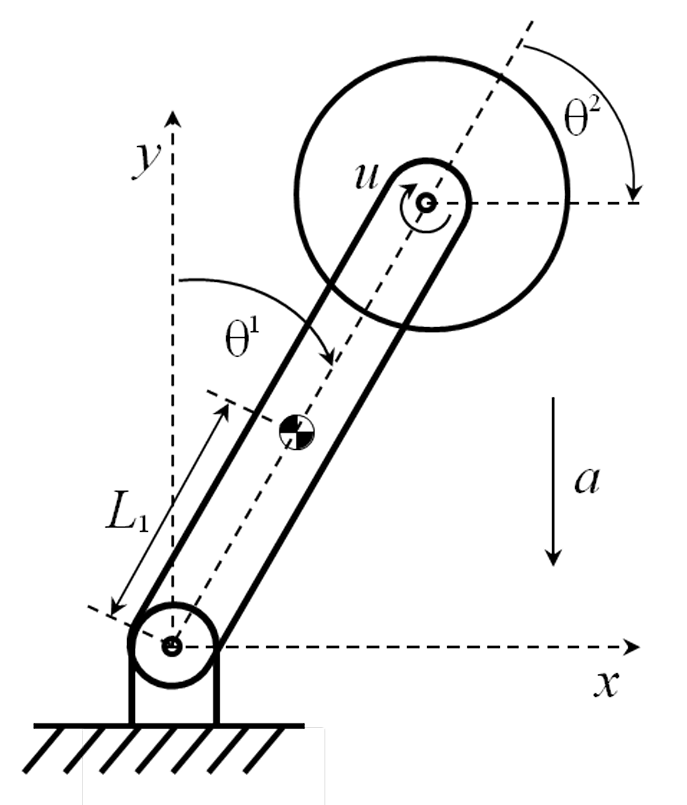
\includegraphics[width=0.4\textwidth]{../Figures/inertia_wheel.png}
    \caption{Inertia Wheel Pendulum}
  \end{figure}
\end{frame}

\begin{frame}{TORA System}

  \begin{figure}
    \centering
    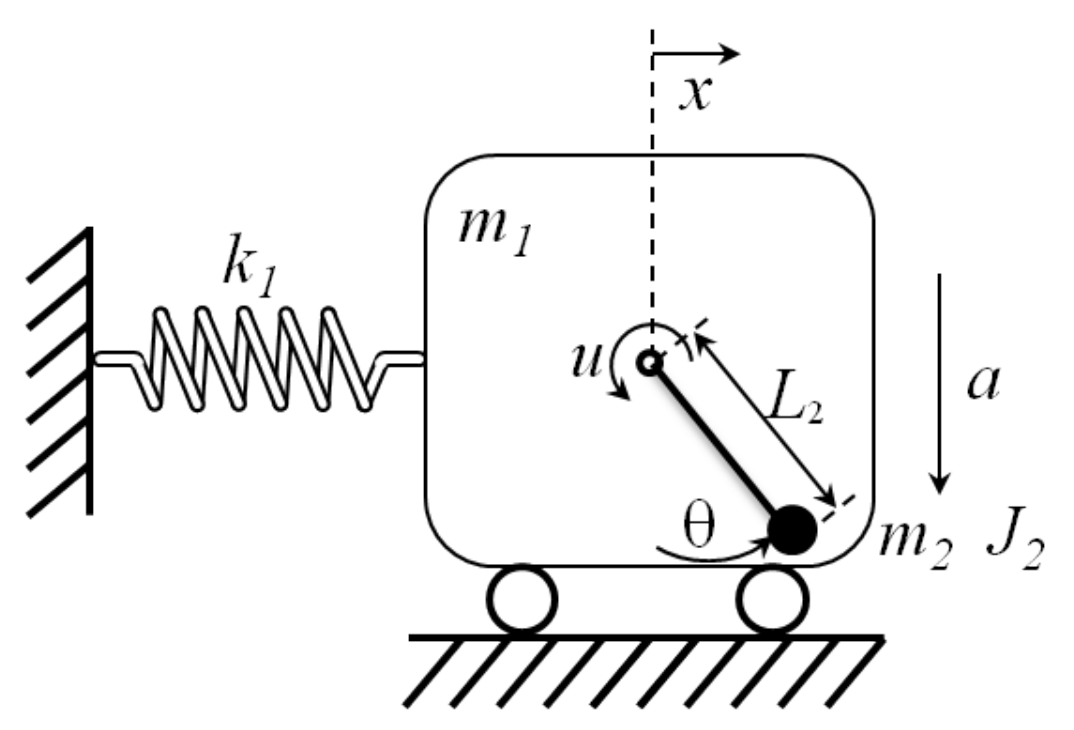
\includegraphics[width=0.4\textwidth]{../Figures/tora.png}
    \caption{Translational Oscillator with Rotational Actuator}
  \end{figure}
  
\end{frame}



\end{document}